\section{Thermal imaging theory}
\label{sec:theory}
The story of infra-red imaging started in 1800, when Herschel discovered 
infra-red radiation experimentally at long wavelengths just outside the visible 
spectrum of sun light.
The quantitative explanation of incandescent infra-red radiation in 1900 by Max 
Planck started a development, which today has resulted in modern infra-red 
technologies with infra-red camera systems- These are also the result of 
scientific developments in semiconductor physics and micro-system 
technologies.\cite{10.1117/12.2266142}\\
Since its birth, it is possible to recognize three generations of infra-red 
cameras\cite{thermalimage}: the first generation cameras were characterized by 
a single element detector, combined with two scanning mirrors to create 
infra-red images. 
Their main disadvantage was that they suffered from saturation problems. 
Saturation indicates the limit of the highest irradiation that can be measured 
by a detector. For digital sensors, since incident photoelectrons are converted 
in charges, each detector can store a maximum amount of charges known as the 
full well capacity.\cite{10.1117/12.2266142}\\
The second generation cameras were characterized by an increase in the number 
of detectors, positioned in a large linear array or in two small 2-D array.
The third generation cameras, i.e., the ones currently used, are characterized 
by large focal plane array (FPA) detectors, thus increasing the reliability 
and sensitivity of such infra-red systems.\cite{rogalski2000infrared} 
%
\subsection{Electromagnetic radiation}
\label{ssec:electromagnetic-radiation}
Electromagnetic radiation is all around (and within, and throughout) us and is
comprised of everything from gamma radiation on the high frequency end to radio
waves on the low frequency end. So the Figure (\ref{fig:spectrum}) give an
overview of EM waves, ordered according to their wave-length or frequency. 
This spectrum consists of a great variety of different waves. All of them can
be observed in nature, and many have technical applications. Starting from the
left of the figure, for example, $\gamma$-rays have the highest frequencies,
that is, the shortest wavelengths.\cite{vollmer2017infrared} \hfill \break
%
%
\begin{figure}[htb]
	\centering
	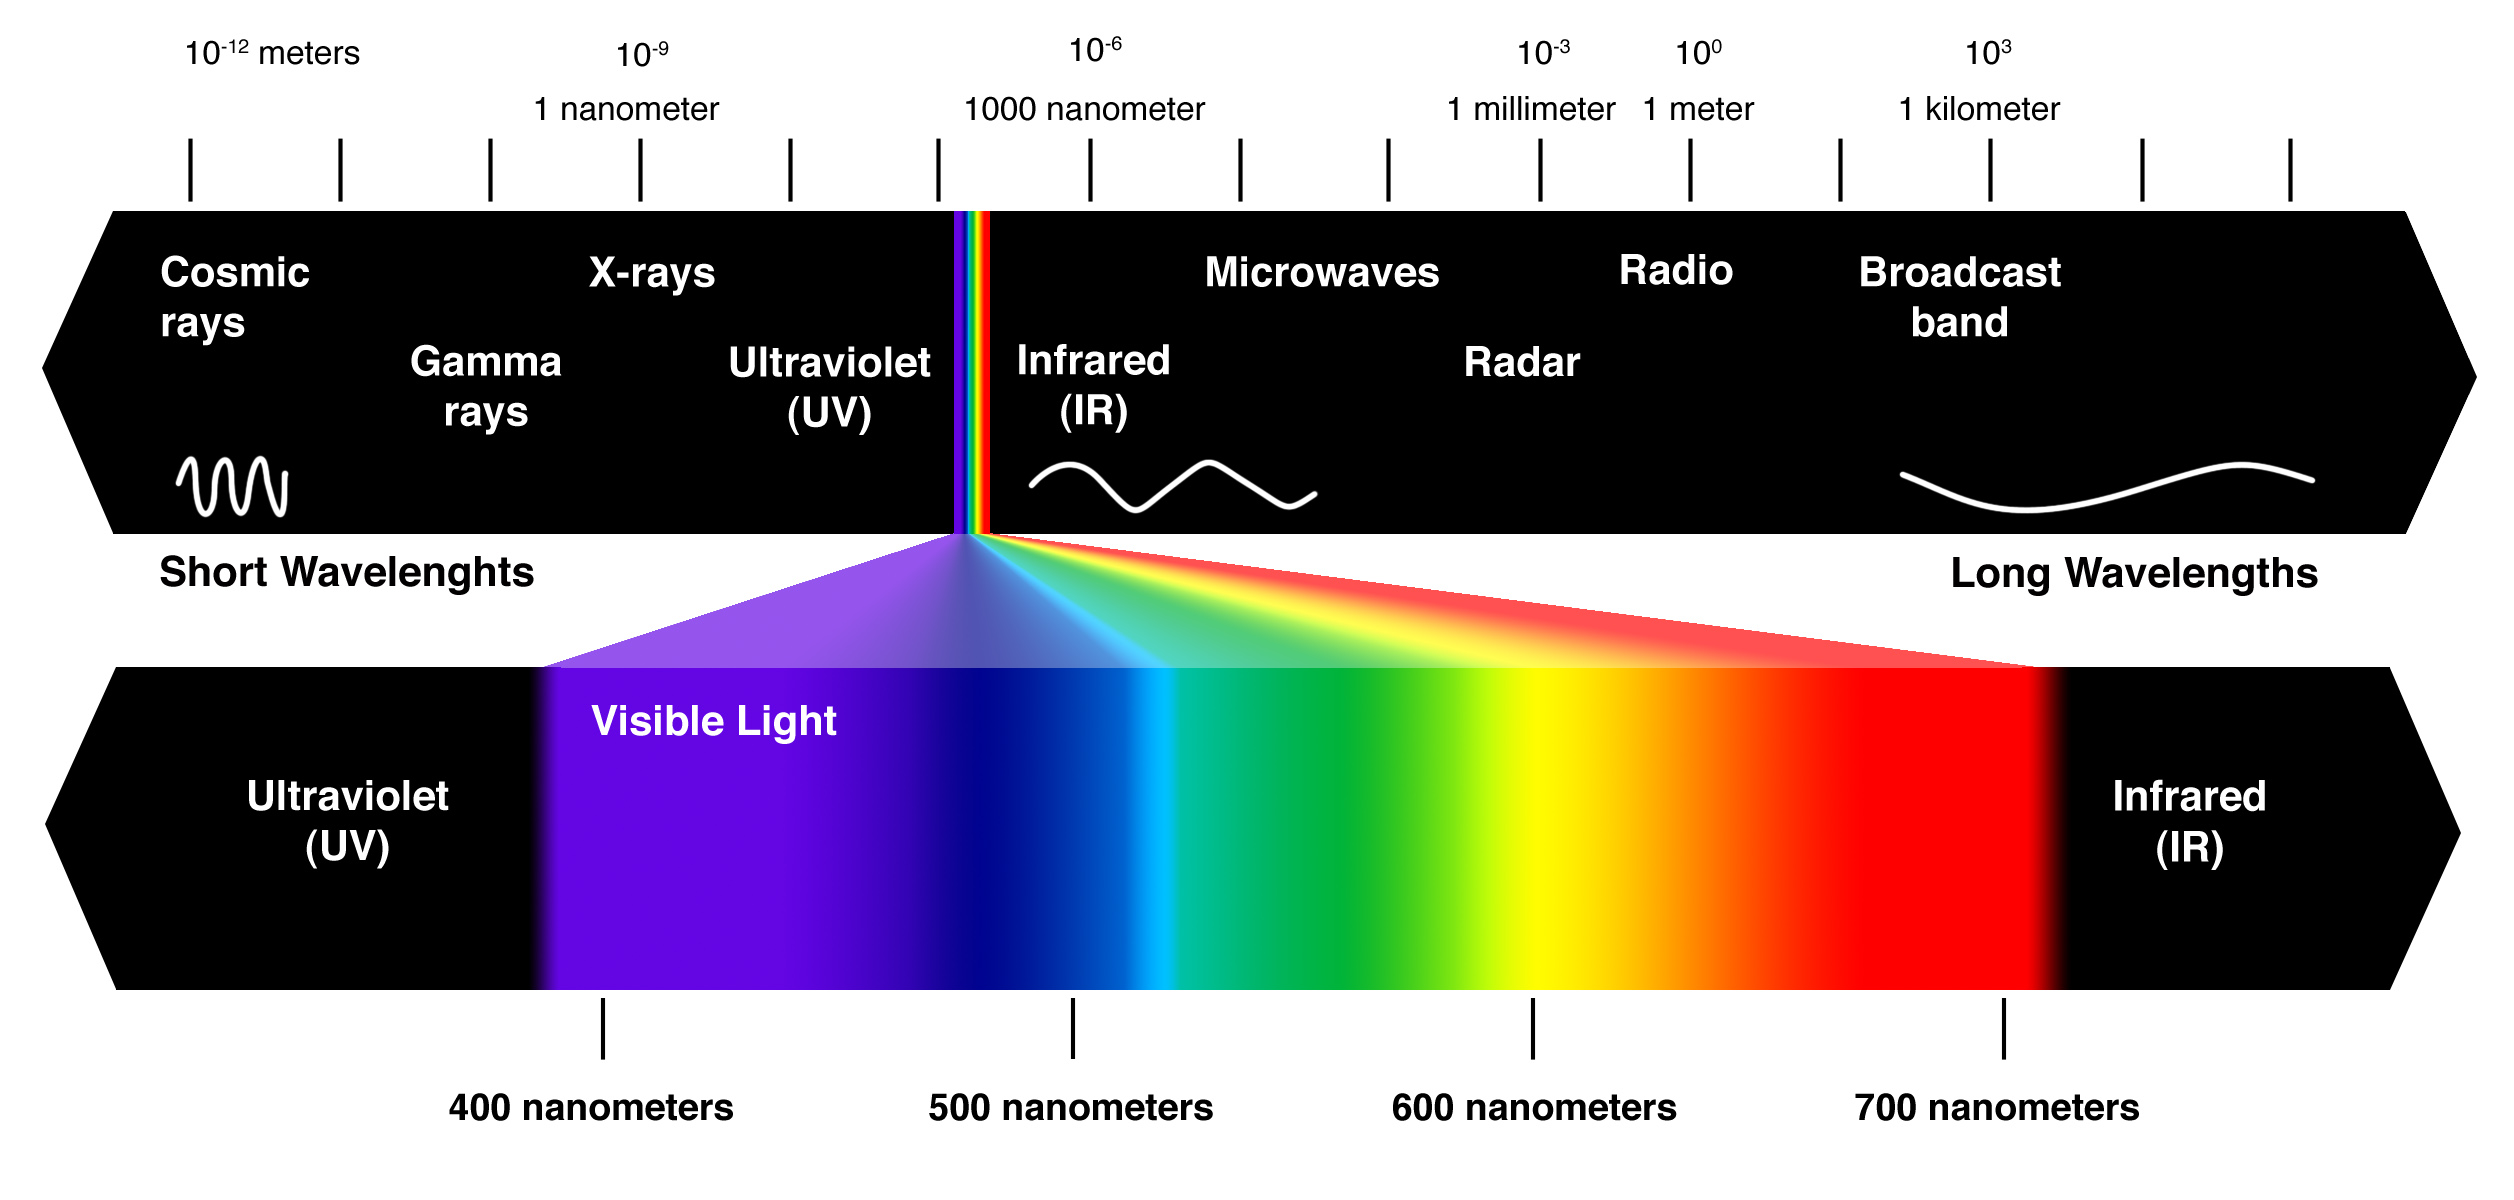
\includegraphics[width=0.75\textwidth]{Visible-spectrum.jpeg}
	\captionsource{Composition of the spectrum of electromagnetic waves.}{
	\href{https://socratic.org/questions/what-is-the-wavelength-of-a-photon-of-blue-light-whose-frequency-is-6-3-10-14-s-}{https://socratic.org}}
	\label{fig:spectrum}
\end{figure}
%
\newline
The visible light, defined by the sensitive range of the light receptors in our
eyes, only covers a very small range within this spectrum, with wavelengths from
$380$ to $780$ \si{\nano\meter}. The adjacent spectral region with wavelengths
from $780$ \si{\nano\meter} up to $1$ \si{\milli\meter} is usually called infra-red. 
This range is followed by microwaves, RADAR, and all EM waves that are used for
radio, TV, and so on.
While most imaging sensors detect radiation in the visible spectrum (wavelengths
from $380$ to $700 \,\si{\nano\meter}$), long wave infra-red sensors detect
radiation the infra-red spectrum, and it accounts for most of the thermal
radiation emitted by objects near room temperature. Then for IR imaging, only a
small range of the IR spectrum is used. 
It is shown in an expanded view in Figure (\ref{fig:spectrum-ir}). \hfill \break 
Typically, three spectral ranges are defined for thermography:
\begin{inparadesc}
\item[\textbf{long-wave (LW)}] region from around $8$ to $14$ \si{\micro\meter}, 
\item[\textbf{mid-wave (MW)}] region from around $3$ to $5$ \si{\micro\meter}, 
\item[\textbf{short-wave (SW)}] region from $0.9$ to $1.7$ \si{\micro\meter}.
\end{inparadesc}
%
%
\begin{figure}[!h]
	\centering
	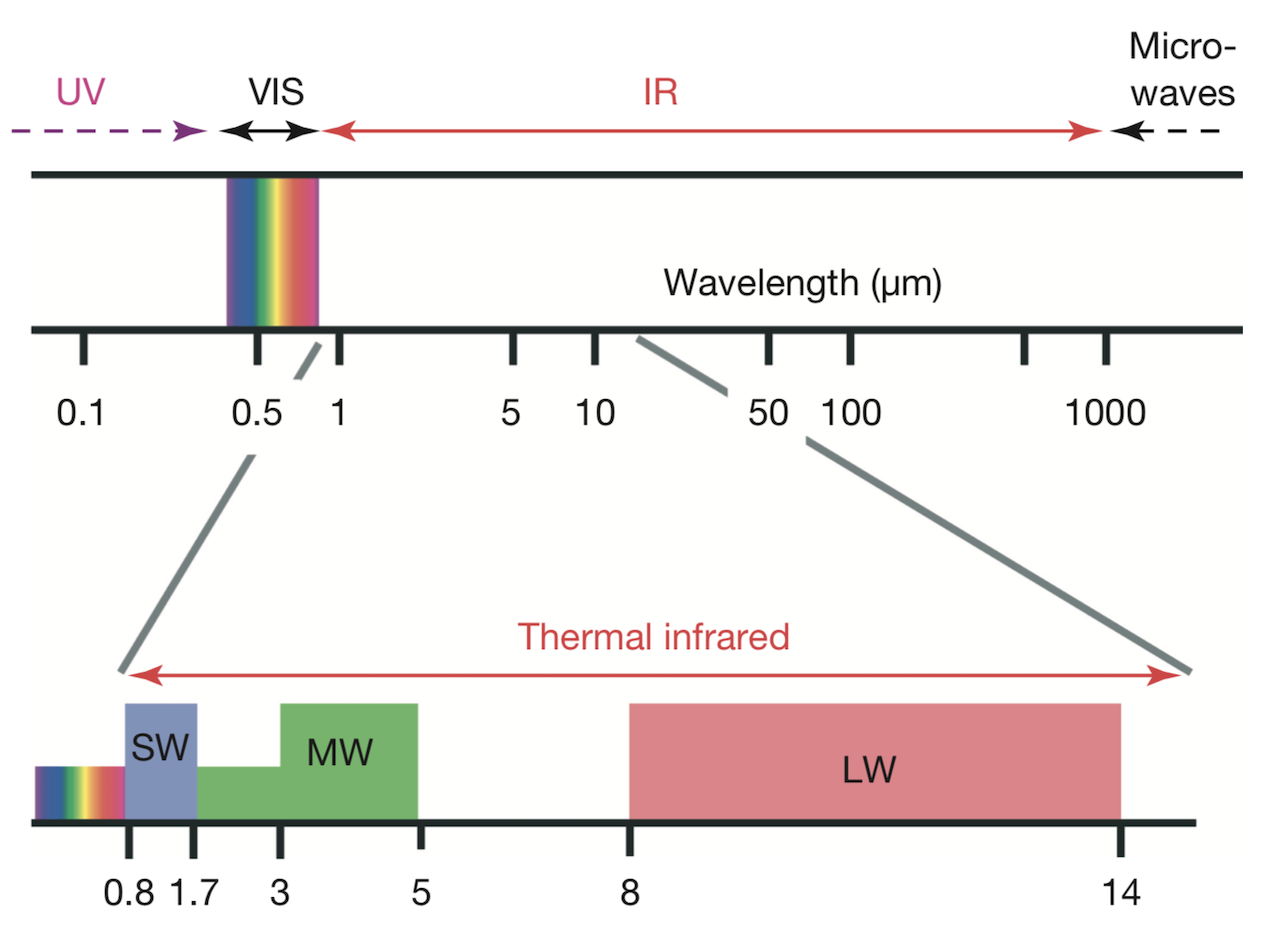
\includegraphics[width=0.65\textwidth]{spectrum-ir.png}
	\captionsource{Infrared (IR) and adjacent spectral regions and expanded view of so-called thermal IR. This is the region where IR imaging systems for short-wave (SW), mid-wave (MW), and long- wave (LW) cameras exist. Special systems have extended ranges.
}{\cite{vollmer2017infrared}}
	\label{fig:spectrum-ir}
\end{figure}
% 
\newline The origin of naturally occurring EM radiation is manifold. 
The most important phenom for thermography is the thermal radiation. 
In brief, the thermal radiation implies that every body or object at a
temperature T $>0 \,$ \si{\kelvin} $\,(-273.15 \,$\si{\celsius}$)$ emits EM
radiation. 
The amount of radiation and its distribution as a function of wavelength depend
on temperature and material properties.\cite{vollmer2017infrared}
For temperatures in the range of natural and technological processes, this 
radiation is in the thermal IR spectral region. 
This is known as the infra-red spectrum, and it accounts for most of the
thermal radiation emitted by objects near room temperature.
%
\subsection{Modern detectors}
\label{ssec:modern-detect}
The main difference between a thermal imaging and normal image capturing is the
sensor used. One type of the sensor used in thermal cameras is called a
microbolometer. Essentially its functionality is similar to the CMOS or CCD
sensor, just in different wavelengths. Unlike many other thermal sensor the
microbolometer doesn't need an active cooling system to function a long period
of times. Modern uncooled detectors use sensors whose working mechanism is based
on a change of resistance, voltage or current when heated by IR radiation.
Uncooled detectors are mostly composed by pyroelectric and ferroelectric
materials or based on microbolometer technology. The thermal signal depends upon
the radiant power but not upon its spectral content, i.e., it is wavelength
independent.\cite{10.1117/12.2266142,rogalski2000infrared}
